\documentclass[]{book}
\usepackage{lmodern}
\usepackage{amssymb,amsmath}
\usepackage{ifxetex,ifluatex}
\usepackage{fixltx2e} % provides \textsubscript
\ifnum 0\ifxetex 1\fi\ifluatex 1\fi=0 % if pdftex
  \usepackage[T1]{fontenc}
  \usepackage[utf8]{inputenc}
\else % if luatex or xelatex
  \ifxetex
    \usepackage{mathspec}
  \else
    \usepackage{fontspec}
  \fi
  \defaultfontfeatures{Ligatures=TeX,Scale=MatchLowercase}
\fi
% use upquote if available, for straight quotes in verbatim environments
\IfFileExists{upquote.sty}{\usepackage{upquote}}{}
% use microtype if available
\IfFileExists{microtype.sty}{%
\usepackage{microtype}
\UseMicrotypeSet[protrusion]{basicmath} % disable protrusion for tt fonts
}{}
\usepackage[margin=1in]{geometry}
\usepackage{hyperref}
\hypersetup{unicode=true,
            pdftitle={Text Mining Techniques for Knowledge Extraction from Technical Documents},
            pdfauthor={Filippo Chiarello},
            pdfborder={0 0 0},
            breaklinks=true}
\urlstyle{same}  % don't use monospace font for urls
\usepackage{natbib}
\bibliographystyle{apalike}
\usepackage{longtable,booktabs}
\usepackage{graphicx,grffile}
\makeatletter
\def\maxwidth{\ifdim\Gin@nat@width>\linewidth\linewidth\else\Gin@nat@width\fi}
\def\maxheight{\ifdim\Gin@nat@height>\textheight\textheight\else\Gin@nat@height\fi}
\makeatother
% Scale images if necessary, so that they will not overflow the page
% margins by default, and it is still possible to overwrite the defaults
% using explicit options in \includegraphics[width, height, ...]{}
\setkeys{Gin}{width=\maxwidth,height=\maxheight,keepaspectratio}
\IfFileExists{parskip.sty}{%
\usepackage{parskip}
}{% else
\setlength{\parindent}{0pt}
\setlength{\parskip}{6pt plus 2pt minus 1pt}
}
\setlength{\emergencystretch}{3em}  % prevent overfull lines
\providecommand{\tightlist}{%
  \setlength{\itemsep}{0pt}\setlength{\parskip}{0pt}}
\setcounter{secnumdepth}{5}
% Redefines (sub)paragraphs to behave more like sections
\ifx\paragraph\undefined\else
\let\oldparagraph\paragraph
\renewcommand{\paragraph}[1]{\oldparagraph{#1}\mbox{}}
\fi
\ifx\subparagraph\undefined\else
\let\oldsubparagraph\subparagraph
\renewcommand{\subparagraph}[1]{\oldsubparagraph{#1}\mbox{}}
\fi

%%% Use protect on footnotes to avoid problems with footnotes in titles
\let\rmarkdownfootnote\footnote%
\def\footnote{\protect\rmarkdownfootnote}

%%% Change title format to be more compact
\usepackage{titling}

% Create subtitle command for use in maketitle
\newcommand{\subtitle}[1]{
  \posttitle{
    \begin{center}\large#1\end{center}
    }
}

\setlength{\droptitle}{-2em}

  \title{Text Mining Techniques for Knowledge Extraction from Technical Documents}
    \pretitle{\vspace{\droptitle}\centering\huge}
  \posttitle{\par}
    \author{Filippo Chiarello}
    \preauthor{\centering\large\emph}
  \postauthor{\par}
      \predate{\centering\large\emph}
  \postdate{\par}
    \date{2018-09-05}

\usepackage{booktabs}

\begin{document}
\maketitle

{
\setcounter{tocdepth}{1}
\tableofcontents
}
\chapter{Introduction}\label{introduction}

\section{Goal}\label{goal}

Il problema non è sostituire domain knowledge. Idea vecchia ha fallito.
E' insostibuibile perchè:

\begin{itemize}
\tightlist
\item
  Technology, interessa gli ingegneri
\item
  Social Science, decision making
\end{itemize}

PErchè fallita: da una parte è andata avanti la knowledge
rappresentation. E' impossibile rappresentare la conoscenza con regole,
ma con altri strumenti si può rappresentare (bottom-up).

Inoltre ho text mining, capaità di processare testi. Parte di
intelligenza artificiale. Questi fenomeni non sostituioscono l'esperto
ma ne cambiano il modo di operare.

Oggi si integra. Vogliamo un esperto di dominio che faccia meglio il suo
mestiere.

Abbiamo oggi più potenza e correzione errori.

Oltre ad efficienza e potenza nel correggere gli errori. Ora c'è anche
la possibilità dio maggiore specificità. L'obiettivo è qiuindi poratre
domain knowledge sia su technology sia ai decisori sociali.

\section{Problem}\label{problem}

Foresight

\section{Solutions}\label{solutions}

\begin{figure}

{\centering 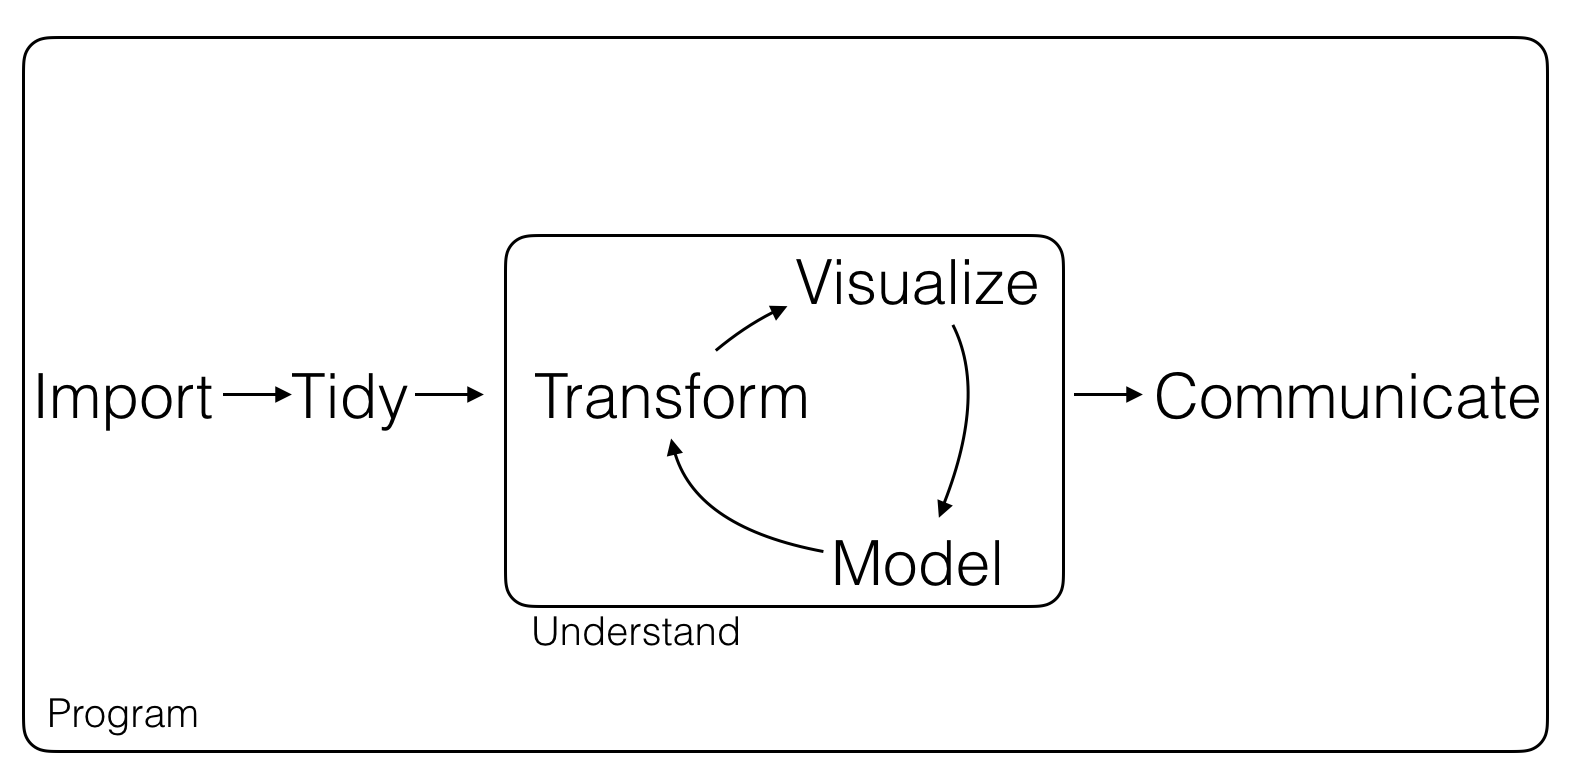
\includegraphics[width=0.8\linewidth]{_bookdown_files/figures/main_work_flow} 

}

\caption{A general workflow for the process of data analysis. Readapted from Wickham (2016)}\label{fig:mainworkflow}
\end{figure}

\section{Challenges: Understanding and
Programming}\label{challenges-understanding-and-programming}

\subsection{Understanding}\label{understanding}

\subsection{Programming}\label{programming}

\section{Research Questions}\label{research-questions}

\section{Stakeholders}\label{stakeholders}

Marketing

Research and Development

Design

Human Resources

Other Stakeholders

\section{Knowledge Intensive Manegement
Engineering}\label{knowledge-intensive-manegement-engineering}

Tipicamente occupaimo di attività ad altà ripetitività. Ti porti dietro
metodologie ingegneristiche applicate a sistemi inernti, andnano a
operare in sistemi socio-tecnici. Hai fatto il tuo mestieri (ricerca
operativa ecc..). Negli ultimi anni però le aziende le attività a
maggior valore aggiunto sono non ripetitive. Innovazione, marketing
ecc.. e quindi gestione della conoscena. Su situazione che sembrano
uniche il gestionale rischia di perdere rispetto al creativo. Come
disciplina voglio presidiare queste aree: non ci occupaimo di casi
unici, ma costruire modelli in grado di incorporare conoscenza per
essere usati in questi. La tesi ha l'obbiettivo di esploration and
exploitation queste direzioni.

\chapter{State of the Art}\label{sota}

The analysis of technical documents require the design of processes that
rely both on programming and Natural Language Processing techniques and
on the undestanding and knowldege of field experts. While the first
techniques are codified and explicit, the second are sometimes implicit
and always harder to systematize. In this section i treat these two
groups of techniques in the same way to give to the reader a sistematic
litterature review on these topics. For this reason the sections of this
chapter has the sequent structure:

\begin{itemize}
\tightlist
\item
  At a first level we have two sections \ref{sotatools} and
  \ref{sotadocuments}, reviewing respectivelly the processes of
  \emph{programming and Natural Language Processing} and of
  \emph{undestanding and knowldege of field experts application};
\item
  Section \ref{sotatools} has a subsection for each of the \emph{phases}
  showed in figure \ref{fig:mainworkflow}. These subsections goes from
  \ref{sotatoolsprogram} to \ref{sotatoolscomunicate};
\item
  Each subsection from \ref{sotatoolsprogram} to
  \ref{sotatoolscomunicate} contains the relative Natural Language
  Processing \emph{task} that are relevant for the analysis of technical
  documents, for example Document Retrieval
  \ref{sotatoolsimportretrieval}, Part-Of-Speech-Tagging;
  \ref{sotatoolstransformpos} or Named Entity Recognition
  \ref{sotatoolsmodelner}.
\item
  Each task subsection describes the relevant \emph{techniques} to
  perform that task. I use the word techniques to include mainly
  algorythms and procedures but also more generic methods or frameworks;
\item
  Since the second section \ref{sotadocuments} describes less
  systematics phases, task and techniques this section opens with a
  first subsection \ref{sotadocumentsunderstand} that focuses on the
  studies of the problems of using expert knowledge in an analytical
  process and which are the techniques to convert this knowledge in a
  format that is usable in a Natural Language Processing workflow.
\item
  Finally, always section \ref{sotadocuments} has a subsection for each
  of the technical \emph{documents} I analyzed (aggiungi gancio con
  introduzione). These subsections goes from \ref{sotadocumentspatents}
  to \ref{sotadocumentsjobs}.
\end{itemize}

\section{Phases, Tasks, and Techniques}\label{sotatools}

In this section I make a review of the most important techniques for
Natural Language Processing in the context of technical documents
analysis. The techniques (mainly algorythms) are grouped in phases
(Import, Tidy, Transform, Model, Visualize, Communicate) showed in
figure \ref{fig:mainworkflow} and each phases is dived in the NLP tasks
that are the most important for the analysis of technical documents. The
algorythms i reviewed in this section are summmarised in table tot,
where the reader can see the relationship between tasks and techniques.

\subsection{Program}\label{sotatoolsprogram}

\begin{itemize}
\tightlist
\item
  \textbf{Articoli Emily}
\end{itemize}

\subsection{Import}\label{sotatoolsimport}

\begin{itemize}
\tightlist
\item
  I tipi di codifica di testo
\item
  Pachetti per import
\end{itemize}

\subsubsection{Document Retrieval}\label{sotatoolsimportretrieval}

\begin{itemize}
\tightlist
\item
  Letteratura query
\end{itemize}

\subsection{Tidy}\label{sotatoolstidy}

\begin{itemize}
\tightlist
\item
  Hadley
\end{itemize}

DTM

problems such as sparsity

\subsection{Transform}\label{sotatoolstransform}

Transforming in the context of Natural Language Processing is what in
computational linguistic is called text normalization. Normalizing text
means converting it to a more convenient, standard form. Most of the
task of technical document analysis in fact relies on first separating
out or tokenizing sentences and words, strip suffixes from the end of
the word, determining the root of a word or transform the text using
regular expressions.

\subsection{Sentence Splitting}\label{sentence-splitting}

The analysis of technical documents require as first process, that the
input text is segmented in sentences. Since documents do not encode this
information in a non ambiguous manner (using dots) due to common
abbreviations (e.g.: ``Mr., Dr.''), a sentence splitting process that
does not rely only on a trivial \emph{dot based} rule is required. This
issue in the technical documents domain is even more problematic due to
the presence of formulas, numbers, chemical entity names and
bibliographic references. Furthermore, since sentece splitting is one of
the first processes of an NLP pipeline, errors in this early stage are
propagated in the following steps causing a strong decrease for what
concerns their accuracy. One of the most advanced techniques are machine
learning techniques: given a training corpus of properly segmented
sentences and a learning algorithm, a statistical model is built. By
reusing the statistical model, the sentence splitter is able to split
sentences on texts not used in the training phase. ItalianNLP lab
systems uses this approach
\citep{dell2009ensemble, attardi2009reverse, attardi2009accurate}. For
this reason this algorythm is used for the most of the application
presented in this Thesis.

\subsection{Tokenization}\label{tokenization}

Since documents are unstructured information, these has to be divided
into linguistic units. The definition of linguistic units is
non-trivial, and more advanced techniques can be used (such as n-gram
extraction) but most of the times these are words, punctuation and
numbers. English words are often separated from each other by
whitespace, but whitespace is not always sufficient. Solving this
problems and splitting words in well-defined tokensis defined as
tokenization. In most of the application described in the present
Thesis, the tokenizer developed by the ItalianNLP lab was integrated
\citep{dell2009ensemble, attardi2009reverse, attardi2009accurate}. This
tokenizer is regular expression based: each token must match one of the
regular expression defined in a configuration file. Among the others,
rules are defined to tokenize words, acronyms, numbers, dates and
equations.

\subsubsection{Stemming}\label{sotatoolstransformstemming}

Stemming is a simpler but cruder methodology for chopping off of
affixes. The goal of stemming is reducing inflected (or sometimes
derived) words to their word stem, base or root form. The stem of a word
and its morphological root do not need to be identical; it is sufficient
that related words map to the same stem, even if this stem is not a
valid root. One of the most widely used stemming is the simple and
efficient Porter algorithm \citep{porter1980algorithm}.

\subsubsection{Lemmatisation}\label{sotatoolstransformlemmatisation}

Lemmatization is the task of determining the root of a words. The output
allow to find that two words have the same root, despite their surface
differences. For example, the verbs \emph{am}, \emph{are}, and \emph{is}
have the shared lemma \emph{be}; the nouns \emph{cat} and \emph{cats}
both have the lemma \emph{cat}. Representing a word by its lemma is
important for many natural language processing tasks. Lemmatisation in
fact diminish the problem of sparsity of document-word matrix.
Futhermore lemmatisaion is important for document retrieval
\ref{sotatoolsimportretrieval} web search, since we want to find
documents mentioning motors if we search for motor. The most recent
methods for lemmatization involve complete morphological parsing of the
word \citep{hankamer1989morphological}.

\subsubsection{N-Grams}\label{sotatoolstransformngrams}

\subsubsection{Part-of-Speech Tagging}\label{sotatoolstransformpos}

The part of speech plays an central role in technical document analysis
since it provides very useful information concerning the morphological
role of a word and its morphosyntactic context: for example, if a token
is a determiner, the next token is a noun or an adjective with very high
confidence. Part of speech tags are used for many information extraction
tools such as named entity taggers (see section \ref{sotatoolsmodelner})
in order to identify named entities. In typical named entity task these
are people and locations since tokens representing named entities follow
common morphological patterns (e.g.~they start with a capital letter).
For the application to technical documents, technical entities (like the
possibile failures of a manufact) becomes more relevant. In this context
a correct part-of-speech tagger becomes even more important since we can
not rely on morphosyntactical rules. In addition part of speech tags can
be used to mitigate problems related to polysemy since words often have
different meaning with respect to their part of speech (e.g. ``track'',
``guide''). This information is extremelly valuable in patent analysis,
and some patent tailored part-of-speech tagger has been designed (see
section \ref{sotadocumentspatents}). The litterature on pos-tagger is
huge, and goes behoind the scope of the present thesis to make a
complete review. In most of the application presentend in this work,was
employed the ILC postagger \citep{attardi2006experiments}. This
postagger uses a supervised training algorithm: given a set of features
and a training corpus, the classifier creates a statistical model using
the feature statistics extracted from the training corpus.

\subsubsection{Regular Expressions}\label{sotatoolstransformregex}

Regular expression (regex) is a language for specifying text search
strings, an algebraic notation for characterizing a set of strings. This
language whidelly used in modern word processor and text processing
tools.. They are particularly useful for searching in texts, when we
have a pattern to search for.

A pattern could be at A regular expression search function will search
through the corpus, returning all texts that match the pattern. The
corpus can be a single document or a collection. For example, the Unix
command-line tool grep takes a regular expression and returns every line
of the input document that matches the expression. A search can be
designed to return every match on a line, if there are more than one, or
just the first match. In the following examples we generally underline
the exact part of the pattern that matches the regular expression and
show only the first match. We'll show regular expressions delimited by
slashes but note that slashes are not part of the regular expressions.

\subsection{Model}\label{sotatoolsmodel}

Classi di modelli. Pedro Domingos

\subsubsection{Document Classification}\label{sotatoolsmodeldocclass}

\subsubsection{Network Analysis}\label{sotatoolsmodelnetanal}

\subsubsection{Sentiment Analsysis}\label{sotatoolsmodelsentanal}

\subsubsection{Named Entity Recognition}\label{sotatoolsmodelner}

\subsubsection{Vector Semantics}\label{sotatoolsmodelvec}

\subsubsection{Topic Modelling}\label{sotatoolsmodeltopicmodel}

\subsection{Visualize}\label{sotatoolsvisualize}

\subsection{Comunicate}\label{sotatoolscomunicate}

\section{Documents}\label{sotadocuments}

\subsection{Understand}\label{sotadocumentsunderstand}

Expertise (collins)

Sheela Jasanow

Taleb?

\subsubsection{The problem of byases}\label{sotadocumentsunderstandbyas}

\subsubsection{The Importance of Lexicons for Technical Documents
Analysis}\label{sotadocumentsunderstandlexicons}

\subsection{Patents}\label{sotadocumentspatents}

\subsection{Papers}\label{sotadocumentspapers}

\begin{itemize}
\tightlist
\item
  Parte Barilari.Keyword base, defini i confini di area tecnologica.
  Hot-topics su paper (guaiè)
\item
  Biblio
\end{itemize}

\subsection{Projects}\label{sotadocumentsprojects}

\subsection{Wikipedia}\label{sotadocumentswiki}

\subsection{Twitter}\label{sotadocumentstwitter}

\subsection{Job Profiles}\label{sotadocumentsjobs}

\chapter{Methods}\label{methods}

In this chapter I describe the methods applied for the analysis of
different types of documents containing technical information. The
methods are ensamble of Natural Language Processing (NLP) and Text
Mining techniques described in @ref(sota\_tools), re-designed depending
on the analyzed document and the analysis goal.

Table tot summarise the relations between the documents under analysis
(introduced in section @ref(sota\_documents)) and the NLP techniques.

Table documents vs tools

Table algorithms vs tools

\section{Patents}\label{patents}

\section{Papers}\label{papers}

\section{Projects}\label{projects}

\section{Wikipedia}\label{wikipedia}

\section{Twitter}\label{twitter}

\section{Job Profiles}\label{job-profiles}

\chapter{Applications and Results}\label{applications-and-results}

Some \emph{significant} applications are demonstrated in this chapter.

\section{Patents}\label{patents-1}

\section{Papers}\label{papers-1}

\section{Projects}\label{projects-1}

\section{Wikipedia}\label{wikipedia-1}

\section{Twitter}\label{twitter-1}

\section{Job Profiles}\label{job-profiles-1}

\chapter{Future Developments}\label{future-developments}

\section{Marketing}\label{marketing}

\section{Research and Development}\label{research-and-development}

\section{Design}\label{design}

\section{Human Resources}\label{human-resources}

\chapter{Conclusions}\label{conclusions}

We have finished a nice thesis

\chapter{Glossary}\label{glossary}

Morphology= the study of the way words are built up from smaller
meaning-bearing units called morphemes.

\bibliography{papers.bib}


\end{document}
